\subsection{3D print design}
The physical enclosure of the wristband was designed and prototyped using 3D printing. This approach enabled rapid iteration and made it possible to adapt the design throughout the development process.

The enclosure was designed to securely house the electronic components while keeping the overall dimensions as compact as possible. Particular attention was given to the placement of the emergency button to ensure that it is easily accessible without being prone to accidental activation.

The enclosure consists of two parts: a base that holds the dev board and battery, and a top cover that protects the components while allowing interaction with the button. Openings for charging and ventilation were minimized to improve durability and support future waterproofing considerations.

\begin{figure}[H]
    \centering
    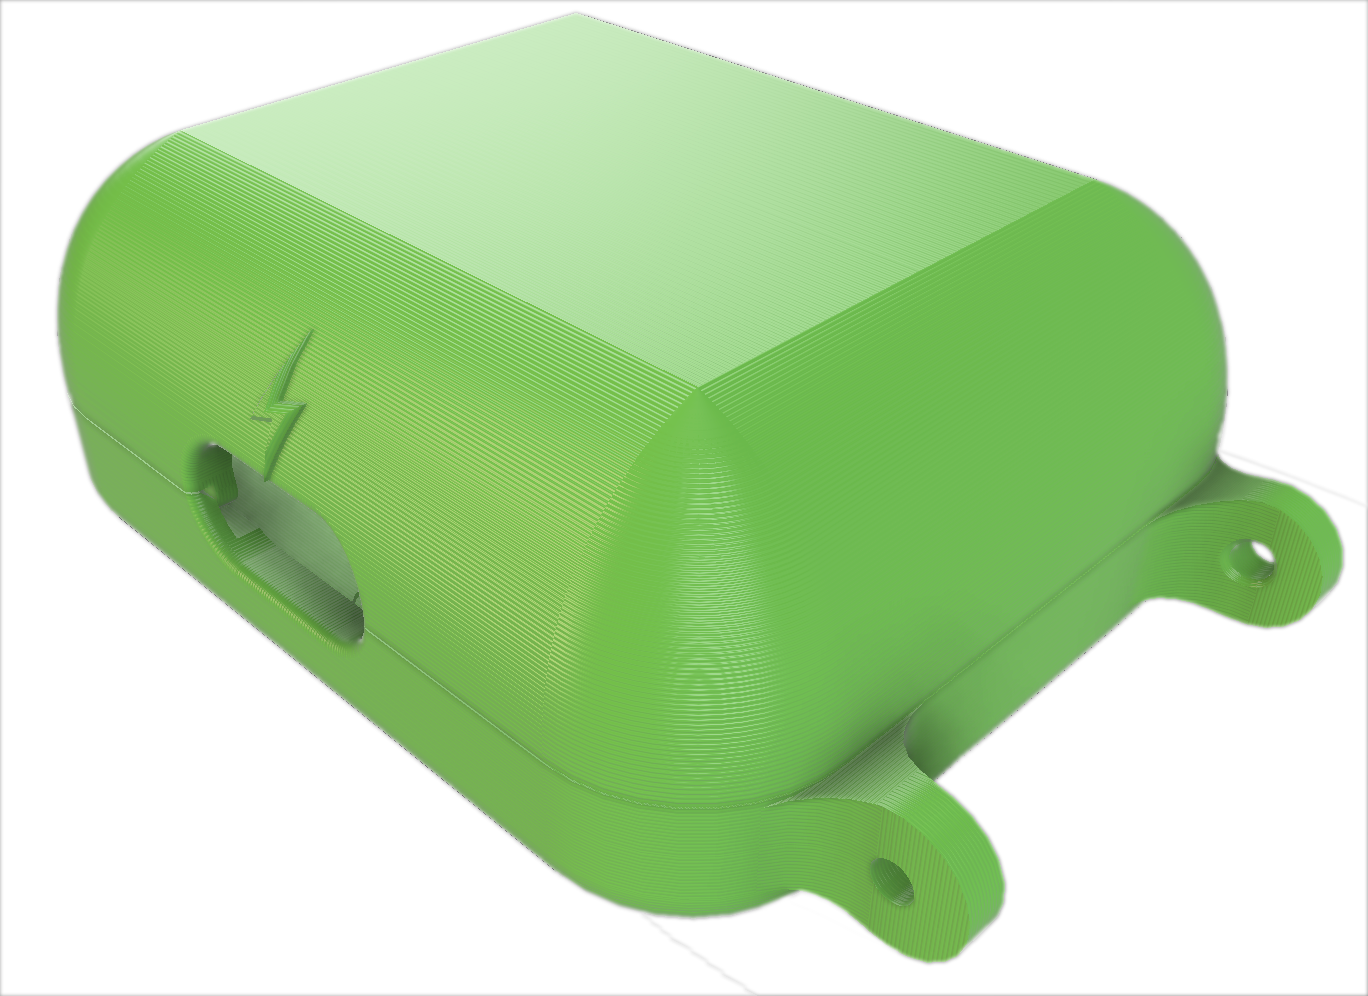
\includegraphics[width=0.5\linewidth]{report//images/Enclosure B.png}
    \caption{Wristband Enclosure}
    \label{fig:wristband_enclosure}
\end{figure}

The use of 3D printing allowed quick adjustments to tolerances and dimensions based on assembly testing. This proved especially valuable when fitting the battery and ensuring sufficient space for wiring and connectors.

